\documentclass[conference]{IEEEtran}
\IEEEoverridecommandlockouts
% The preceding line is only needed to identify funding in the first footnote. If that is unneeded, please comment it out.
\usepackage{cite}
\usepackage{amsmath,amssymb,amsfonts}
\usepackage{algorithmic}
\usepackage{graphicx}
\usepackage{minted}
\usepackage{textcomp}
\usepackage{xcolor}
\usepackage{polski}
\usepackage{comment}
\usepackage[utf8]{inputenc}
\usepackage{graphicx}
\def\BibTeX{{\rm B\kern-.05em{\sc i\kern-.025em b}\kern-.08em
    T\kern-.1667em\lower.7ex\hbox{E}\kern-.125emX}}
\begin{document}

\title{Implementacja gry planszowej "Chińczyk"}

\author{\IEEEauthorblockN{Adam Hyjek}
\IEEEauthorblockA{\textit{nr indeksu: 234987} \\
\textit{Politechnika Wrocławska}\\
Wrocław, Polska \\
}
\and
\IEEEauthorblockN{Bartosz Rodziewicz}
\IEEEauthorblockA{\textit{nr indeksu: 226105} \\
\textit{Politechnika Wrocławska}\\
Wrocław, Polska \\
}
}

\maketitle


\section{Streszczenie}
Celem projektu jest stworzenie aplikacji pozwalającej na rozegranie gry planszowej "Chińczyk" (znanej także jako "Ludo" oraz "Człowieku, nie irytuj się") na pojedynczym komputerze. W skład aplikacji umożliwiającej przeprowadzenie rozgrywki we wspomnianej grze wchodzi zarówno logiki sterującej grą, jak i graficzny interfejs użytkownika, co umożliwi komfortową rozgrywkę w czasie rzeczywistym. Aplikacja zostanie zaimplementowana w języku GDScript zaprojektowanym specjalnie na potrzeby silnika Godot \cite{godot}.

\section{Wstępny opis słowny}
Zadaniem aplikacji jest umożliwienie rozegrania partii gry "Chińczyk". W tym celu po jej uruchomieniu ekranie wyświetla się plansza zawierająca składająca się z czterdziestu pól, czterech domków oraz czterech schowków. Ponadto na planszy znajduje się 16 pionków, po 4 w każdym z 4 kolorów reprezentujących poszczególnych graczy oraz kostka do gry. Na ekranie wyświetla się także krótka instrukcja do obsługi programu oraz wskazanie na gracza mającego właśnie kolejkę \cite{wiki}.\par
Aplikacja umożliwia kolejnym graczom wykonanie swojej kolejki poprzez wykonanie rzutu kostką oraz, w przypadku posiadania legalnego ruchu, wybór pionka, którym zostanie wykonany ruch.  Ponadto program umożliwia przeprowadzenie podstawowych działań składających się na reguły gry takich jak bicie, wprowadzanie pionków do domków, wyprowadzanie pionków ze schowka, ponowienie rzutu po wyrzuceniu "szóstki", czy wykrycie końca rozgrywki w momencie wprowadzenia wszystkich pionków do domku przez jednego z graczy. Dodatkowo aplikacja powinna implementować funkcjonalności usprawniające doświadczenie użytkownika. Jedno z takich funkcjonalności jak menu ustawień umożliwiające dostosowanie ustawień graficznych, zmianę liczby graczy, czy zmianę sposobu sterowania. Kolejnymi funkcjami możliwymi do zaimplementowania są obsługa myszy do przesuwania pionków, animacja ich przesuwania, a także możliwość gry z komputerem. Ponadto aplikacja powinna posiadać menu początkowe oraz ekran zakończenia gry wskazujący zwycięzcę.

\newpage
\section{Słownik pojęć z dziedziny problemu}
Słownik został opracowany na podstawie zasad gry opisanych w \cite{wiki}.
\begin{itemize}
    \item Bicie - Sytuacja, w której pionek jednego koloru wkracza na pole zajmowane przez pionek innego koloru. W takiej sytuacji pionek, który uprzednio zajmował dane pole zostaje "zbity" i powraca do schowka.
    \item Domek - Cztery pola będące docelową lokalizacją pionków danego gracza. Gracz ma prawo wprowadzić pionka do domku dopiero po okrążeniu nim całej planszy, do domku jednego gracza nie mogą wejść pionki innego gracza (koloru). W momencie, w którym jeden z graczy zapełni swój domek wszystkimi swoimi pionkami wygrywa grę.
    \item Gracz - Jedna z czterech osób uczestniczących w grze. Każdy gracz posiada swój unikalny kolor i cztery pionki. Podczas swojej kolejki gracz rzuca kością i decyduje, który pionek zostanie ruszony. W grze uczestniczy czterech graczy.
    \item Kolejka - Moment, w którym dany gracz może wykonać swój ruch. Gracze wykonują swój ruch po kolei, zgodnie ze wskazówkami zegara. Kolejka składa się z rzutu kostką i przesunięcia pionka. W momencie, gdy gracz wyrzucił na kości "szóstkę" powtarza ruch przed zakończeniem kolejki.
    \item Kość - Służy do losowego określenia liczby pól, o które gracz przesunie pionka. Efektem rzutu kością jest liczba oczek z zakresu 1-6.
    \item Kolor - Unikalny identyfikator każdego z graczy określający jego pionki, schowek, pole startowe oraz domek.
    \item Pionek - Figura, którą porusza gracz podczas swojej kolejki w celu przesunięcia jej do domku. Każdy z graczy ma cztery pionki o własnym kolorze i po umieszczeniu wszystkich w domku wygrywa grę.
    \item Plansza - Miejsce rozgrywania gry. Składa się z czterdziestu pól, w tym czterech startowych, czterech domków oraz czterech schowków.
    \item Pole - Część planszy, po której można przesuwać pionki w celu okrążenia planszy i umieszczenia ich w domku. Na planszy znajduje się 36 zwykłych pól oraz 4 pola startowe.
    \item Pole startowe - Cztery pola, na których umieszcza się pionki po wyprowadzeniu ich ze schowka. Każde z pól posiada własny kolor odpowiadający kolorowi gracza posiadającego schowek.
    \item Schowek - Miejsce startowe wszystkich pionków. Celem gracza jest wyprowadzenie tych pionków poprzez wyrzucenie "szóstki" na kości i umieszczenie pionka na odpowiednim polu startowym. Istnieją cztery schowki, po jednym dla każdego gracza.
    \item Ruch - Moment przesunięcia pionka po rzucie kością. Zazwyczaj gracz w jednej kolejce wykonuje jeden ruch, wyjątkiem jest sytuacja, w której gracz wyrzucił "szóstkę" - wtedy po wykonaniu ruchu w nagrodę ponownie rzuca kością i wykonuje dodatkowy ruch przed zakończeniem kolejki.
\end{itemize}


\section{Analiza wymagań użytkownika}
Aplikacja ma za zadanie umożliwienie przeprowadzenia rozgrywki w grę "Chińczyk". W tym celu z punktu widzenia użytkownika aplikacja musi wykonywać dwie czynności: rzut kością do gry oraz wykonanie ruchu wskazanym przez gracza pionkiem o liczbę oczek określoną wykonanym przed ruchem rzutem. W ramach każdego wykonywanego ruchu program musi sprawdzić jego legalność i zabronić wykonywania ruchów niedozwolonych, takich jak ruch pionkiem ze schowka w momencie wyrzucenia mniejszej liczby oczek niż 6. Oprócz tego gra musi być wstanie wykryć i wykonać sytuację bicia pionka (gdy pionek gracza najedzie na pole, na którym znajduje się pionek przeciwnika) i osiągnięcie warunku zwycięstwa w postaci umieszczenia wszystkich pionków w domku. W formie graficznej wymagania te obrazuje diagram przypadków użycia:
\hspace*{-2cm}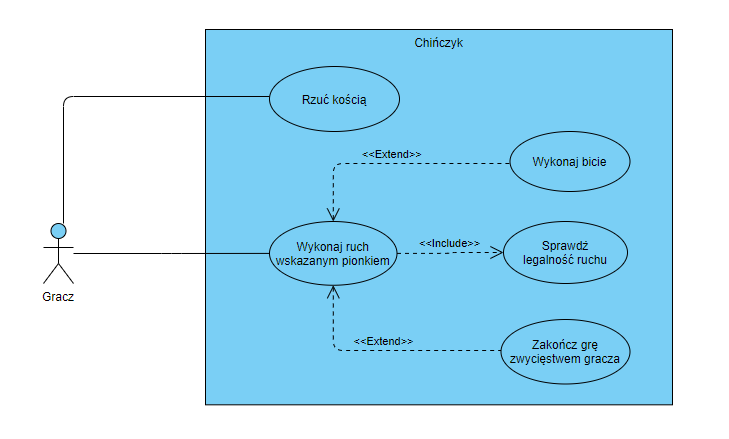
\includegraphics[scale=0.60]{UseCase.PNG} \par
Aktor w postaci gracza może wykonać dwie podstawowe czynności: rzut kością lub wykonanie ruchu wybranym pionkiem. Integralną częścią wykonywanego ruchu jest sprawdzenie jego legalności, stąd związek zawierania pomiędzy omawianymi przypadkami użycia. W przypadku wykonywania bicia oraz zakończenia gry, te przypadki użycia nie będą występować przy każdym wykonaniu ruch, więc są z nim w związku rozszerzenia.

\section{Modele systemu z różnych perspektyw}
Model systemu zakłada istnienie czterech klas reprezentujących cztery kluczowe pojęcia ze słownika opisującego dziedzinę problemu. Są to: plansza, kość do gry, gracz oraz pionek. Taki podział umożliwia reprezentację wszystkich kluczowych pojęć w możliwie najprostszej formie.\par
Plansza do gry jest rozbudowaną klasą opisującą i przeprowadzającą rozgrywkę. Zawiera ona wszystkich graczy oraz położenia ich pionków, a także ma dostęp do kości do gry. Ponadto zawiera on zmienne niezbędne do kontrolowania stanu rozgrywki określające stan gry, stan tury, rezultat ostatniego rzutu kostką i wskazującą gracza oczekującego na swoją kolejkę.\par
Klasa \texttt(Dice) opisująca kość do gry jest prostą klasą przechowującą wygląd kości i umożliwiającą symulowanie jej działania poprzez losowanie liczby z zakresu od 1 do 6 za pomocą funkcji \texttt(rollDice()). Ponadto klasa ta posiada standardową funkcję \texttt(\_ready()) wywoływaną w momencie pojawienia się kości na ekranie po raz pierwszy.\par
Kolejną klasą jest przedstawiająca gracza klasa \texttt(Player). Każdy gracz reprezentowany jest poprzez \texttt(id), a ponadto przechowuje informacje o własnych pionkach. Do zadań tej klasy należy zainicjowanie pionków za pomocą funkcji \texttt(spawnPawns()) i kontrola ich położenia - funkcja \texttt(isAnyPawnOnBoard()) służy do określenia, czy któryś z czterech pionków wyszedł ze schowka, a funkcja \texttt(areAllPawnsFinished()) sprawdza warunek zwycięstwa, czyli czy wszystkie pionki znajdują się w domku. \par
Ostatnią niezbędną klasą jest klasa \texttt(PlayerPawn) uosabiająca pionki posiadane przez graczy. Zakłada się, że każdy z pionków ma przypisany do siebie numer \texttt(pawnId) oraz id kontrolującego go gracza (\texttt(playerId)). Ponadto każdy z pionków musi mieć określoną aktualną pozycję (zmienna \texttt(currentPosition)) oraz początkową pozycję (\texttt(startPosition)). Zmienna pawnPlace określa status pionka (w schowku, na planszy, w bazie), a zmienna label przechowuje graficzną reprezentację obiektu. Do określenia pozycji na planszy wykorzystywana jest zmienna \texttt(distanceFromStart), która określa ile pól przebył pionek. Dzięki znajomości całkowitej liczby pól, które pionek musi przebyć przed dotarciem do domku zawsze jesteśmy w stanie precyzyjnie określić jego pozycję na tej trasie. \par \newpage
Graficzną reprezentację powyższego opisu stanowi diagram klas:

\hspace*{-2cm}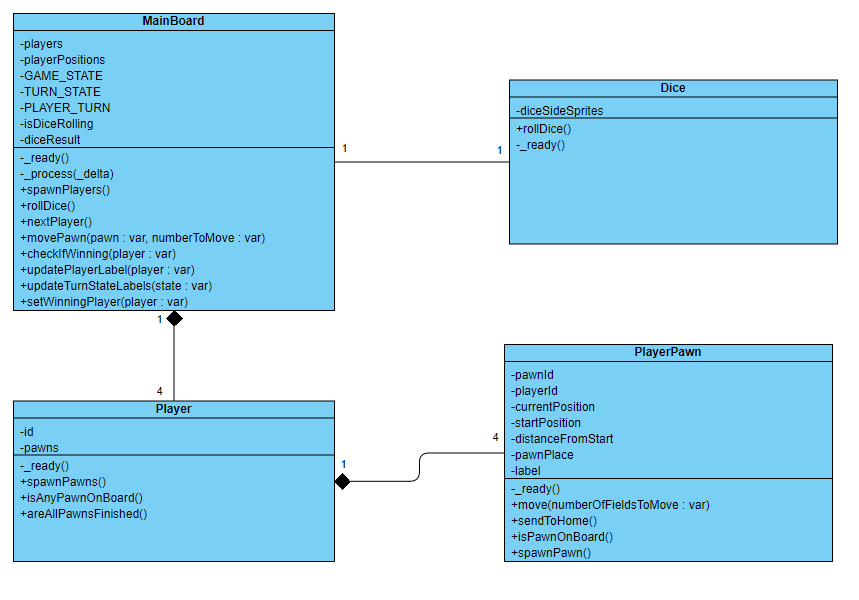
\includegraphics[scale=0.48]{Class.PNG} \par
Główną klasą kontrolującą stan rozgrywki jest klasa \texttt(MainBoard), w związku z tym posiada ona najwięcej relacji z pozostałymi klasami. Jest ona w stanie komunikować się z klasą \texttt(Dice) dzięki związkowi asocjacji o pojedynczej krotności, a ponadto zawiera w sobie obiekty klasy \texttt(Player). W związku z tym obie klasy łączy związek agregacji całkowitej - obiekt klasy \texttt(MainBoard) zawiera cztery obiekty klasy \texttt(Player). Ponadto w aplikacji istnieje związek agregacji całkowitej pomiędzy klasami \texttt(Player) oraz \texttt(PlayerPawn) - każdy obiekt klasy \texttt(Player) zawiera cztery obiekty klasy \texttt(PlayerPawn)

Główną funkcjonalnością programu jest przeprowadzanie rozgrywki w grę "Chińczyk". W tym celu aplikacja musi przyjmować od użytkownika sygnały wejściowe w postaci odpowiednich klawiszy i odpowiednio na nie reagować w zależności od stanu przeprowadzanej rozgrywki. Do monitorowania stanu rozgrywki służą zmienne każdy obiekt klasy \texttt(Player) zawiera cztery obiekty klasy \texttt(GAME\_STATE), \texttt(TURN\_STATE) oraz \texttt(PLAYER\_TURN). Pierwsza zmienna odpowiada za ogólny stan rozgrywki, taki jak: gra jeszcze nie rozpoczęta, gra w trakcie, czy gra zakończona. Zmienna \texttt(PLAYER\_TURN) określa zawodnika, którego kolejka właśnie trwa, z kolei zmienna \texttt(TURN\_STATE) reprezentuje moment tury, w którym obecnie znajduje się program. Jest ona kluczowa dla działania całej aplikacji, ponieważ znacząco wpływa na zachowanie danej iteracji pętli głównej. \newpage
Poniżej przedstawiono diagram sekwencji modelujący pojedynczą iterację pętli głównej odpowiedzialnej za działanie programu:
\hspace*{-0.1cm}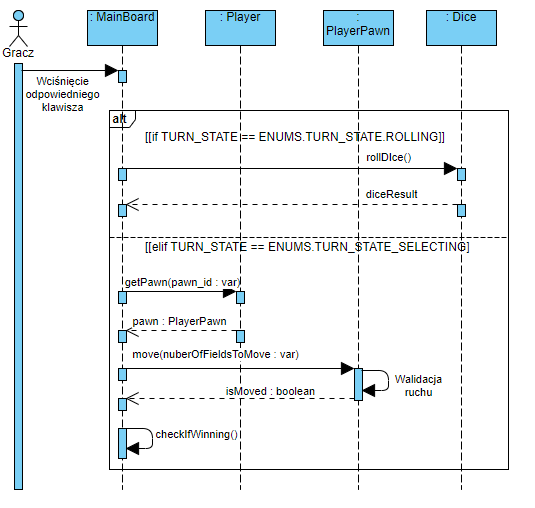
\includegraphics[scale=0.65]{Sequence.PNG} \par
W przypadku gdy stan tury, reprezentowany przez zmienną \texttt(TURN\_STATE) odpowiada wartości \texttt(ENUMS.TURN\_STATE.ROLLING) program jest w fazie poprzedzającej rzut kością. W związku z tym obiekt klasy \texttt(MainBoard) komunikuje się z obiektem klasy \texttt(Dice) poprzez wywołanie funkcji \texttt(rollDice()) zwracającej wynik rzutu kością. Warto wspomnieć, że warunkiem wykonania tej części kodu jest wciśnięcie przez użytkownika klawisza odpowiedzialnego za interakcję, domyślnie jest to spacja. Z kolei jeżeli zmienna \texttt(TURN\_STATE) odpowiada wartości \texttt(ENUMS.TURN\_STATE.SELECTING) program reaguje na klawisze 1-4 odpowiadające poszczególnym pionkom posiadanym przez gracza. Po dokonaniu wyboru obiekt klasy \texttt(MainBoard) rozpoczyna komunikację z odpowiednim obiektem klasy \texttt(Player) w celu otrzymania pionka, który ma zostać przesunięty. Następnie obiekt klasy \texttt(MainBoard) wywołuje funkcję \texttt(move) z argumentem oznaczającym wyrzuconą liczbę oczek, która waliduje żądany ruch i zwraca zmienną binarną określającą, czy ruch jest legalnych i czy zakończył się sukcesem. W takim przypadku następuje sprawdzenie warunku zwycięstwa i zmiana stanu tury.

\section{Kwestie implementacyjne}
Projekt został zaimplementowany na bazie silnika Godot Engine, który jest złożonym, wieloplatformowym narzędziem do tworzenia gier 2D oraz 3D. Umożliwia on w prosty sposób wyeksportować tworzony projekt na najpopularniejsze obecnie systemy operacyjne takie jak Windows, Linux, macOS, Android, iOS, a ponadto na platformy webowe, na przykład HTML. Silnik Godot tworzy kompleksowe środowisko wspierające pełny cykl tworzenia gier, dzięki czemu jest to jedyne narzędzie potrzebne do stworzenia gry "Chińczyk". Godot umożliwia m.in. tworzenie grafiki przy pomocy biblioteki OpenGL ES, wspiera wielokanałowe systemu dźwiękowe a także posiada system ułatwiający tworzenie GUI \cite{godot}.\par
Wybranym językiem programowania został język GDScrpit, który jest językiem skryptowym zintegrowanym z silnikiem Godot. Umożliwia on tworzenie aplikacji wykorzystujących ten silnik wykorzystując przy tym minimalną możliwą ilość kodu co zwiększa produktywność i ułatwia jego naukę. GDScript jest dynamicznie typowanym językiem upraszczający tworzony kod i nie wymagającym kompilacji do jego testowania \cite{godot}.

\section{Podsumowanie i dyskusja krytyczna}
W ramach tego projektu udało nam się zrealizować i zaimplementować niezbędne funkcjonalności systemu umożliwiającego zagranie w grę "Chińczyk". Jedyną rzeczą, której nie udało nam się zaimplementować było ponowienie rzutu kością po wyrzuceniu "szóstki". Pomimo, że projekt można by rozszerzyć o pewne dodatkowe funkcjonalności takie jak menu ustawień, animację pionków, czy możliwość sterowania myszką to nie wpłynęłyby one znacząco na zasadnicze zachowanie systemu, a jedynie polepszyły doświadczenie użytkownika. \par
W procesie tworzenia aplikacji zaznajomiliśmy się z tematyką programowania gier, a także poznaliśmy interesujące, otwartoźródłowe środowisko do ich tworzenia - Godot Engine. Implementuje on specjalny język GDScript usprawniający tworzenie gier komputerowych, dzięki czemu po krótkim zapoznaniu się z jego składnią i dokumentacją silnika mogliśmy skupić się na modelu samej aplikacji.

\section*{Kod źródłowy}
Kod źródłowy zaiplementowanej gry jest dostępny w repozytorium pod adresem: https://github.com/baatochan/LudoGame

\begin{thebibliography}{00}
\bibitem{godot}
Dokumentacja silnika Godot: https://docs.godotengine.org/pl/latest/

\bibitem{wiki}
Strona na Wikipedii objaśniająca zasady gry "Chińczyk": https://pl.wikipedia.org/wiki/Chińczyk\_(gra\_planszowa)

\end{thebibliography}


\end{document}
